
\documentclass[aspectratio=1610]{beamer}

% Can also use "43" or "169" for aspect ratio above

\usetheme[unclass]{LANL}
\usepackage{graphicx}


%% For a classified document, modify the "usetheme" line above:
%\usetheme[myclass=CLASSIFICATION-LEVEL,classcolor=red]{LANL}
%% and add something like this:
%\leftspecial{\color{red}
%    {\bf TYPE OF DATA}\\
%    This document contains {\em blah blah blah} as defined in
%    {\em blah blah blah}.
%    Unauthorized disclosure is subject to {\em blah blah blah}.
%}
%\centerspecial{
%    blah blah blah
%}
%\rightspecial{
%    Classified By: {\em blah blah blah}\\
%    Derived From: {\em blah blah blah}
%}


\usepackage{amsmath}
\usepackage{amsfonts}
\usepackage{amssymb}
%\usepackage{fancyhdr}
%\usepackage[margin=1in]{geometry}
%%\usepackage{graphicx}
%%\usepackage{cite}
\usepackage{multicol}
%%\usepackage[section]{placeins}
%%\usepackage{amsthm}
\usepackage{nicefrac}
\usepackage{bm}
%%\usepackage{algorithm2e}
%\newtheorem{theorem}{Theorem}
%\newtheorem*{theorem*}{Theorem}
%\newtheorem{lemma}{Lemma}
%\newtheorem*{lemma*}{Lemma}
%\newtheorem*{def*}{Definition}
%\newtheorem*{conj}{Conjecture}
%\newtheorem{defn}{Definition}
%\newcommand{\low}[1]{$_{\text{#1}}$}
%\newcommand\xput[2][0.5]{%
%    \rule{#1\linewidth}{0pt}\makebox[0pt][c]{#2}\hfill}
%\usepackage{stackengine}
%\usepackage{enumerate}
\usepackage{tikz}
\usetikzlibrary{arrows.meta}
\usetikzlibrary{decorations.pathreplacing}


\usepackage{epigraph}
\usepackage{booktabs}

\newcommand\tikzmark[2]{
  \tikz[remember picture, overlay]\node[inner sep=0pt] (#1) {#2};}

\usepackage{graphicx}
\usepackage{subcaption}
\usepackage{caption}

\usepackage{colortbl}
\usepackage[absolute,overlay]{textpos}

\usepackage{soul}

\makeatletter
\let\HL\hl
\renewcommand\hl{%
  \let\set@color\beamerorig@set@color
  \let\reset@color\beamerorig@reset@color
  \HL}
\makeatother

\usepackage{cleveref}

%
%\newcommand{\delt}[1]{
%\begin{tikzpicture}[#1]
%\draw (0,0) -- (1ex,1.5ex);
%\draw (2.1ex,0) -- (1ex,1.5ex);
%\draw (0.0,0.0) -- (2.1ex,0);
%\draw (0.5ex,0.8ex) -- (1.5ex, 0.8ex);
%\draw (1ex, 0.75ex) -- (1ex, 0);
%\end{tikzpicture}
%}
\usepackage[all]{xy}


\newcommand{\nhalf}{\nicefrac{1}{2}}
%\newcommand{\eps}{\epsilon_{machine}}
\newcommand{\ol}{\overline}
\renewcommand{\b}{\bm}
%\newcommand{\problem}[2]{ \ \\\textbf{#1} \textit{#2}\\} 
%
\newcommand{\bE}{\mathbb{E}}
\newcommand{\bP}{\mathbb{P}}
\newcommand{\bR}{\mathbb{R}}
\newcommand{\bN}{\mathbb{N}}
\newcommand{\bZ}{\mathbb{Z}}
\newcommand{\bQ}{\mathbb{Q}}
\newcommand{\bC}{\mathbb{C}}
\newcommand{\cA}{\mathcal{A}}
\newcommand{\cB}{\mathcal{B}}
\newcommand{\cC}{\mathcal{C}}
\newcommand{\cD}{\mathcal{D}}
\newcommand{\cE}{\mathcal{E}}
\newcommand{\cF}{\mathcal{F}}
\newcommand{\cG}{\mathcal{G}}
\newcommand{\cH}{\mathcal{H}}
\newcommand{\cI}{\mathcal{I}}
\newcommand{\cJ}{\mathcal{J}}
\newcommand{\cK}{\mathcal{K}}
\newcommand{\cL}{\mathcal{L}}
\newcommand{\cM}{\mathcal{M}}
\newcommand{\cN}{\mathcal{N}}
\newcommand{\cO}{\mathcal{O}}
\newcommand{\cP}{\mathcal{P}}
\newcommand{\cQ}{\mathcal{Q}}
\newcommand{\cR}{\mathcal{R}}
\newcommand{\cS}{\mathcal{S}}
\newcommand{\cT}{\mathcal{T}}
\newcommand{\cU}{\mathcal{U}}
\newcommand{\cV}{\mathcal{V}}
\newcommand{\cW}{\mathcal{W}}
\newcommand{\cX}{\mathcal{X}}
\newcommand{\cY}{\mathcal{Y}}
\newcommand{\cZ}{\mathcal{Z}}

\definecolor{lblue}{RGB}{51,255,255}
\definecolor{dgreen}{RGB}{49,128,23}
\definecolor{nicepink}{RGB}{255, 0, 102}
\definecolor{nicered}{RGB}{255, 80, 80}
\definecolor{lgray}{RGB}{217, 217, 217}
\definecolor{lgreen}{RGB}{77, 255, 166}

\newcommand{\ka}{\kappa}
%
\newcommand{\fp}{\varrho}
\newcommand{\fat}{\mathit{fat}}
\newcommand{\fatr}{\mathit{fat}_{\fp}}
%\renewcommand{\arraystretch}{1.5}
%\renewcommand{\thefootnote}{\fnsymbol{footnote}}	
%\setlength{\headheight}{5pt}
%\pagestyle{fancyplain}
%\renewcommand{\headrulewidth}{0pt}
%\lhead{}
%\chead{}
%\rhead{}
\newtheorem{question}{Question}
%\lfoot{}
%\cfoot{\thepage}
%\rfoot{}

\setbeamerfont{block body}{size=\small}

%\usetheme{Frankfurt}
%\usecolortheme{seahorse}
%\usefonttheme{professionalfonts}

%\setbeamertemplate{navigation symbols}{\insertframenumber/\inserttotalframenumber}
\setbeamertemplate{navigation symbols}{}


\newtheorem{conjecture}{Conjecture}

\institute[LANL]{Los Alamos National Laboratory}


\title{MetConSIN}
\subtitle{}
\author[Brunner]{James D. Brunner, Ph.D.}
\LAUR{}

\makeatletter
\let\@@magyar@captionfix\relax
\makeatother

\usepackage[style=verbose,backend=bibtex]{biblatex}

\addbibresource{allrefs.bib}
\renewcommand{\footnotesize}{\scriptsize}

\begin{document}
\maketitle

\begin{frame}{MetConSIN}

{\scriptsize
Concept:
\begin{itemize}
\item Genome-scale models and constraint based methods are commonly used and allow us to use knowledge of microbial genome sequences to predict metabolic behavior.
\item This modeling paradigm implies a dynamical system that couples optimization with differential equations, and is very difficult to simulate and analyze.
\begin{itemize}\scriptsize
\item Naively, optimization must be done at every time-step.
\item Really, optimization is only required at a (relatively) sparse set of time-points.
\end{itemize}
\item This dynamical system can be understood as a sequence of simpler dynamical systems which model species-metabolite interaction networks.
\end{itemize}

Planned Implementation:
\begin{itemize}
\item Use metagenomic sequencing of environmental samples to build genome scale models of microbial community members.
\item Simulate community genome (metagenome) scale dynamics of metabolism.
\item Identify time intervals of constant network topology \& corresponding networks.
\item Identify impactful transitions in network topology.
\item Develop simplified \& tractable predictive modeling for design \& engineering by leveraging the ``sequence of networks" structure of the microbial community.
\end{itemize}
}
\end{frame}

%--------------------------------------------------------------------------------------------------
\begin{frame}{MetConSIN}
\begin{minipage}{0.45\textwidth}
\begin{center}
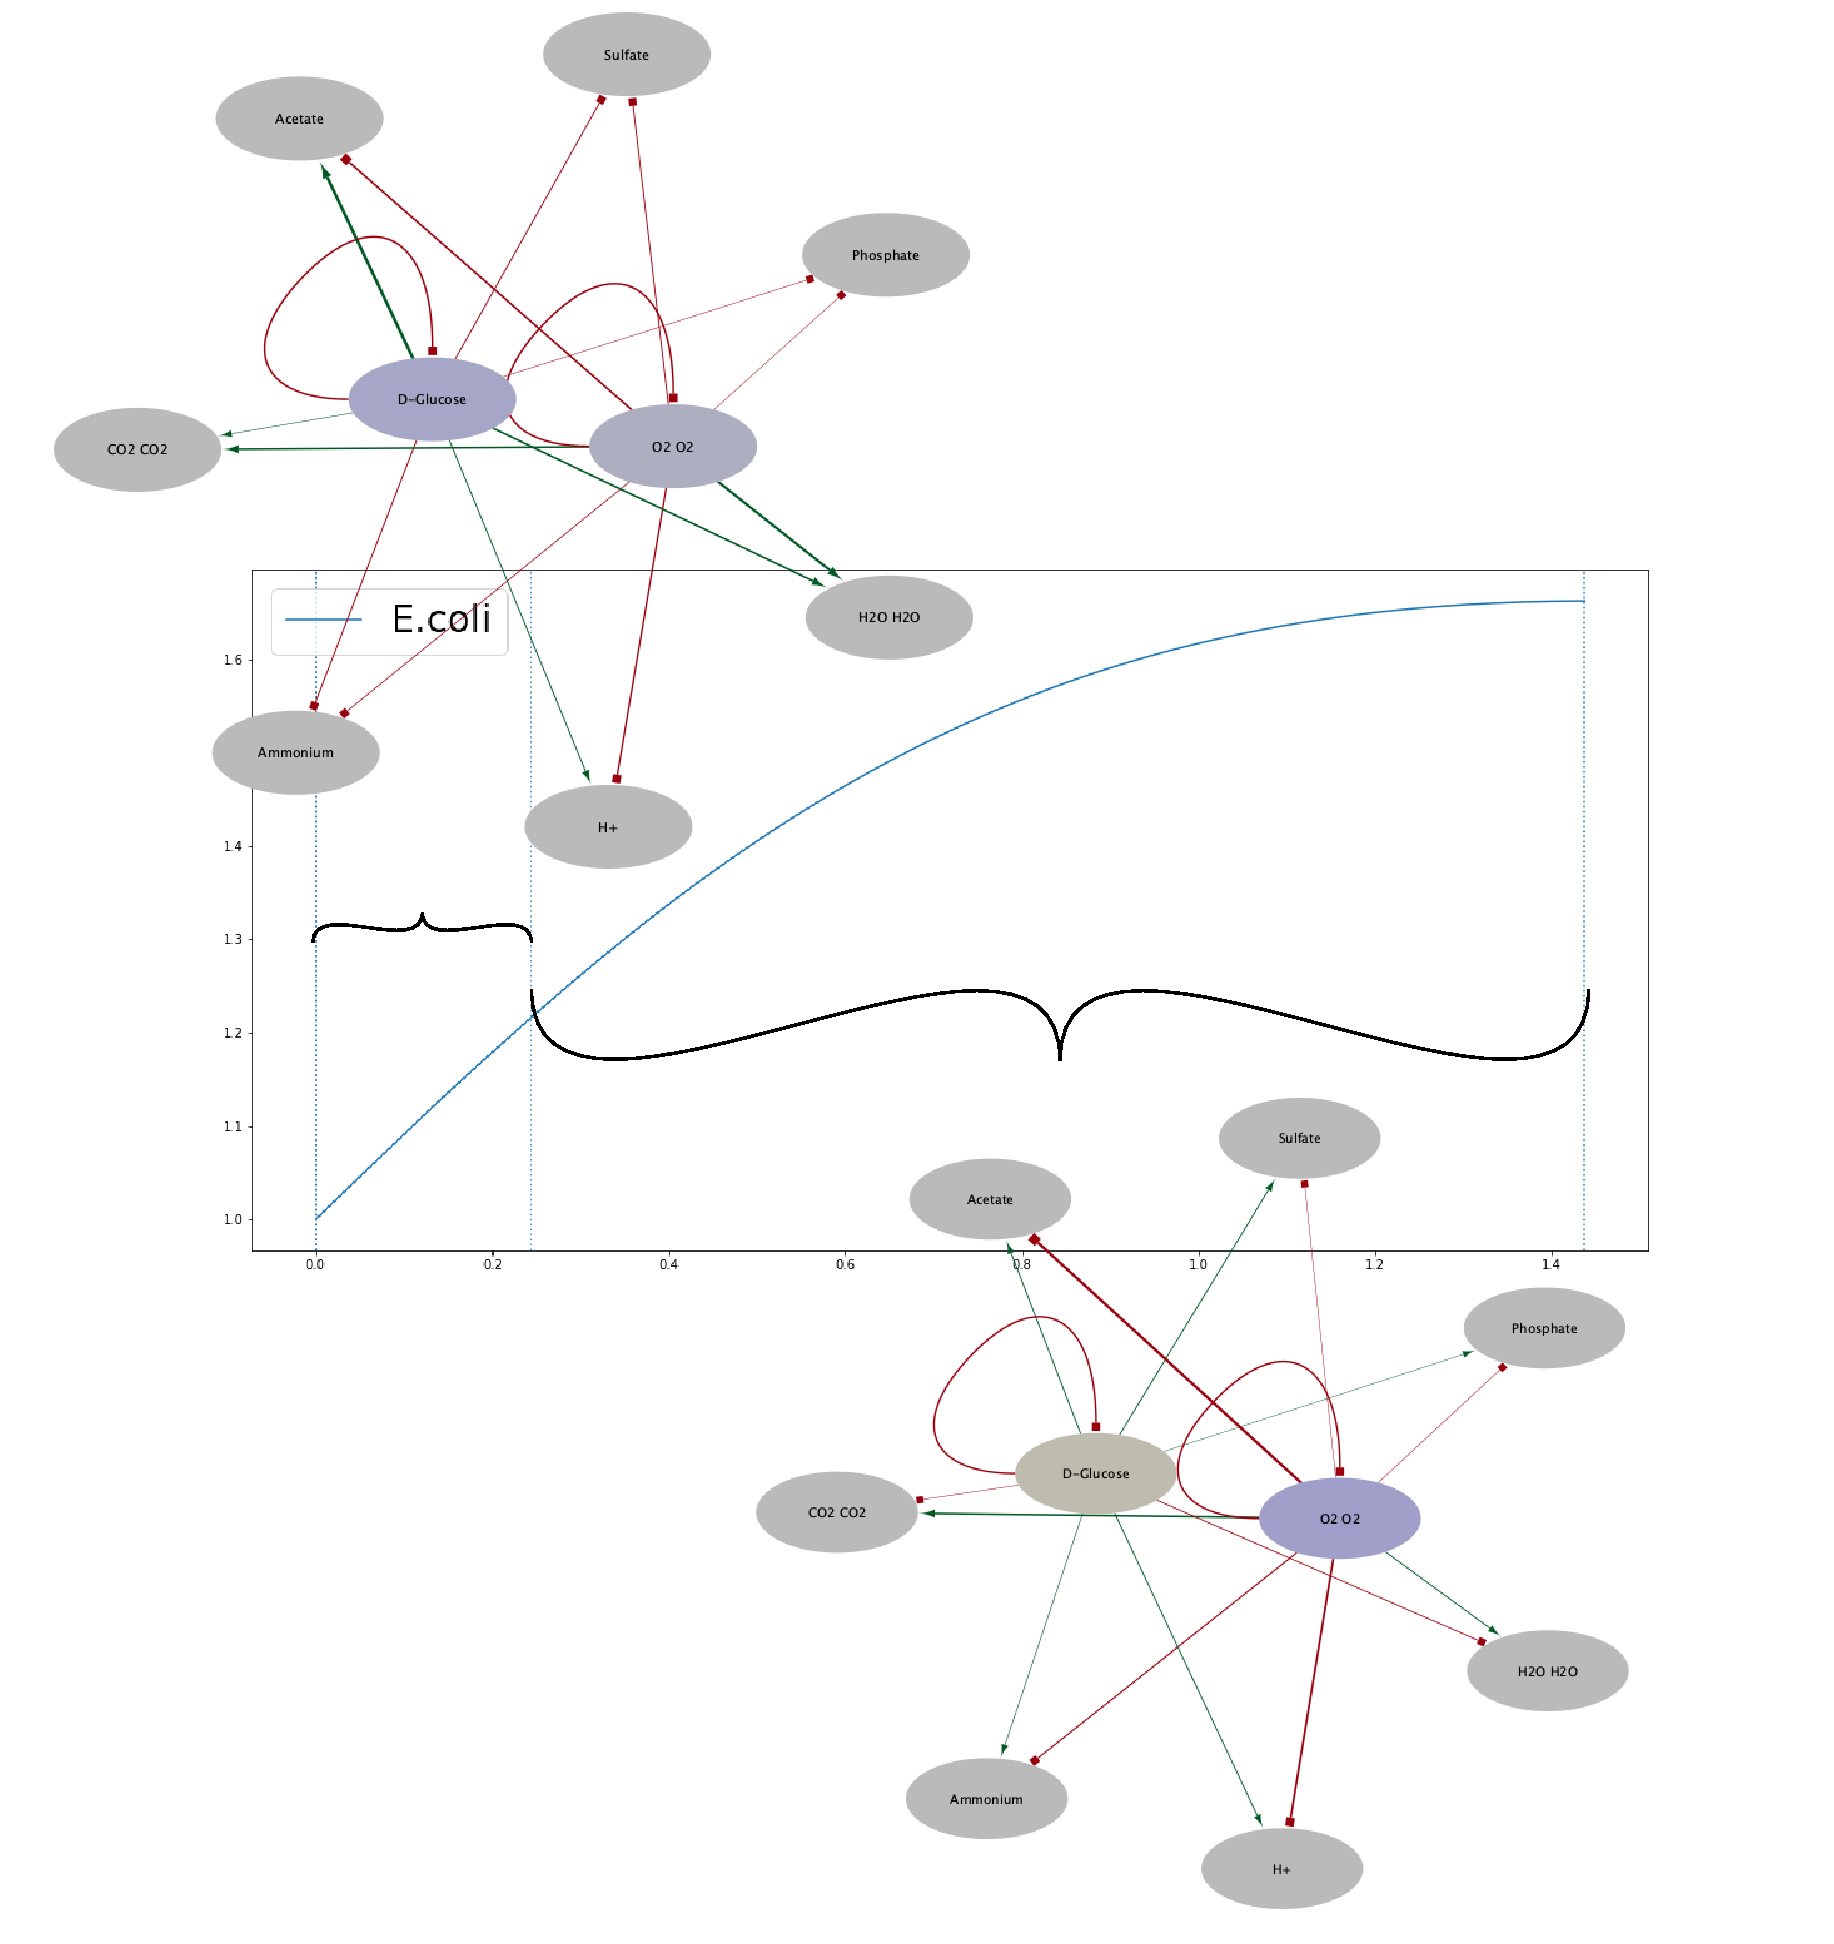
\includegraphics[scale =0.18]{metabolites.pdf}
\end{center}

{\tiny During simulated growth of \emph{E. coli}, we observe two distinct networks of interactions between metabolites (as mediated by \emph{E. coli}).}

\end{minipage}\hspace{1cm}
\begin{minipage}{0.45\textwidth}
\begin{block}{Idea}
Simulating a microbiome (microbes \& external metabolites) using genome scale metabolic models provides a dynamically changing network of interactions.
\end{block}
\vspace{0.4cm}

{\small Using GEMs constructed from metagenomic data, MetConSIN will allow us to

\begin{itemize}
\item Understand the interactions of microbes \& metabolites in a microbiome.
\item Predict \& manipulate microbial community composition.
\item Predict \& manipulate microbiome metabolite production.
\end{itemize}
}
\end{minipage}

\end{frame}
%--------------------------------------------------------------------------------------------------
\end{document}
%%------------------------------------------------------------------------------------------------